\documentclass[xetex,mathserif,serif, 8pt]{beamer}

\usepackage{estilo}
\usetheme{Antibes}
\usecolortheme{beaver}

\title[Simulación de procesadores cuánticos] % (optional, only for long titles)
{Diseño y simulación de procesadores cuánticos que implementen algoritmos cuánticos de busqueda}
\author[M. Casanova] % (optional, for multiple authors)
{Miguel Casanova}
\institute[Universidad Simón Bolívar] % (optional)
{
  Coordinación de Tecnología e Ingeniería Electrónica\\
  Universidad Simón Bolívar
}
%\date[KPT 2004] % (optional)
%{Conference on Presentation Techniques, 2004}
%\subject{Computer Science}

\AtBeginSection[]
{
  \begin{frame}
    \frametitle{Tabla de contenidos}
    \tableofcontents[currentsection]
  \end{frame}
}

\begin{document}

\frame{\titlepage}

\begin{frame}
\frametitle{Estructura de la presentación}
\tableofcontents
\end{frame}

\section{Objetivos}
\begin{frame}
    \frametitle{Objetivo General}

    Diseñar y simular procesadores cuánticos (PC) que implementen los algoritmos cuánticos (AC) de Grover, Shor y PageRank Cuántico (Google Cuántico).

\end{frame}

\begin{frame}
    \frametitle{Objetivos Específicos}

    \begin{enumerate}
        \item Construir la representación circuital cuántica de los AC de Grover, Shor y de Google Cuántico.
        \item Estudiar la dinámica de arquitecturas superconductoras controlables por microondas basadas en transmones.
        \item Precisar la dinámica de secuencias de pulsos necesarios para generar con transmones la compuertas cuánticas necesarias para los AC considerados.
        \item Simular en Mathematica, de forma algebraica, cada una de las arquitecturas de CC considerados.
        \item Simular en Python, de forma numérica, con y sin decoherencia cuántica, el operador evolución de cada una de los compuertas de los CC estudiados.
        \item Comparar los casos con y sin decoherencia cuántica, para cada uno de los AC estudiados, en base a los resultados obtenidos de las simulaciones numéricas y algebraicas.
    \end{enumerate}

\end{frame}

\section{Información cuántica}

\begin{frame}
    \frametitle{Espacios de Hilbert}

    Un espacio de Hilbert es un espacio lineal real o complejo con un producto interno que también define un espacio normado completo.

    \begin{enumerate}
        \item Producto interno
        \item Normado
        \item Completo: Todas las sucesiones de Cauchy convergen fuertemente. Las sucesiones de Cauchy son aquellas en las que el ordenamiento no afecta la convergencia.
        \item Separable: Tiene bases discretas, ortonormales y contables (Tiene dimensión comparable a $\mathds{N}$).
    \end{enumerate}

\end{frame}

\begin{frame}
    \frametitle{Operadores}

    \begin{enumerate}
        \item Operadores hermíticos: $U = U^\dagger$
            \begin{enumerate}
                \item Autovalores reales
                \item Diagonal real
                \item Diagonalizable
            \end{enumerate}
            \vspace{0.5cm}

        \item Operadores unitarios: $U U^\dagger = \mathds{1}$
            \begin{enumerate}
                \item Determinante de módulo igual a la unidad
                \item Preserva normas y trazas
                \item Diagonalizable
            \end{enumerate}
    \end{enumerate}

\end{frame}

\begin{frame}
    \frametitle{Postulados de la mecánica cuántica}

    La QM que fundamenta la teoría de información cuántica se describe formalmente con los siguientes postulados desarrollados por la escuela de Copenhague a lo largo de todo el siglo XX \cite{Cohen_1977}

    \begin{enumerate}
        \item En un tiempo fijo $t_0$, el estado está dado por el ket $\ket{\psi(t_0)}$, perteneciente al espacio de Hilbert $\mathcal{H}$.
        \item Toda cantidad física $\mathcal{A}$, que se pueda medir, está descrita por un operador hermítico $\hat{A}$. Este operador es un observable.
        \item El único resultado posible de una medida de la cantidad física $\mathcal{A}$ es alguno de los autovalores del observable correspondiente $\hat{A}$.
        \item Si un sistema en el estado normalizado $\ket{\psi}$, la probabilidad de obtener un valor $\lambda$ al medir un observable $\mathcal{A}$ está dada por 
            
            \begin{equation}
                p(\lambda) = \sum\limits_i^{g_n} \abs{\braket{\lambda_i}{\psi}}^2
            \end{equation}

            Donde $g_n$ es el grado de degeneración de $\hat{A}$ en $\lambda$, $\ket{\lambda_i}$ son los autoestados asociados a $\lambda$ y el proyector $\Pi_\lambda$ es $\Pi_\lambda = \sum_i^{g_n} \ketbra{\lambda_i}$.
    \end{enumerate}
\end{frame}

\begin{frame}
    \frametitle{Postulados de la mecánica cuántica}

    \begin{enumerate}
        \setcounter{enumi}{4}
        \item Si un sistema físico está en el estado $\ket{\psi}$, el estado resultante luego de una medida ideal del observable $\mathcal{A}$ está dado por

            \begin{equation}
                \ket{\psi} \rightarrow \frac{\Pi_\lambda \ket{\psi}}{\sqrt{\bra{\psi} \Pi_\lambda \ket{\psi}}}
            \end{equation}

        \item La evolución temporal del estado $\ket{\psi(t)}$  está dada por la ecuación de Schrödinger

            \begin{equation}
                i \hbar \frac{d}{dt} \ket{\psi(t)} = \hat{H}(t) \ket{\psi(t)}
            \end{equation}

    \end{enumerate}
\end{frame}

\begin{frame}
    \frametitle{Estados puros y mixtos}

    Las mezclas estadísticas de estados cuánticos, también son estados cuánticos.

    \begin{enumerate}
        \item Estados puros: representados en base al ket $\ket{\psi}$ o a la matriz densidad $\rho = \ketbra{\psi}$.
            \begin{enumerate}
                \item Normalizado: $\braket{\psi} = \int_{-\infty}^{\infty} \abs{\psi(r)}^2 dV = 1$
				\item Traza igual a la unidad: $Tr(\rho) = Tr(\rho^2) = 1$
            \end{enumerate}
            \vspace{0.5cm}

        \item Estados mixtos: representados por $\rho = \sum_i p_i \rho_i$, siendo $\rho_i = \ketbra{\psi_i}$.
            \begin{enumerate}
                \item Matriz hermítica
                \item Traza igual a la unidad
                \item Autovalores no negativos
				\item Traza: $Tr(\rho^2) < 1$
            \end{enumerate}
    \end{enumerate}

    Para estados mixtos se utiliza la ecuación de Liouville-von Neumann.

    \begin{equation}
        i \hbar \dot{\rho}(t) = [\hat{H}, \rho(t)]
    \end{equation}
	
\end{frame}

\begin{frame}
    \frametitle{Sistemas multipartitos}

    Cuando se tiene más de un espacio de Hilbert, el sistema global se forma con el producto tensorial

    \begin{align}
        \mathcal{H} &= \mathcal{H}_A \otimes \mathcal{H}_B \\
        \ket{\psi, \phi} &= \ket{\psi} \otimes \ket{\phi} = \ket{\psi}_A \otimes \ket{\phi}_B \\
        \rho_{AB} &= \rho_A \otimes \rho_B \text{ \  (Estado producto)} \\
        \rho_{AB} &\neq \rho_A \otimes \rho_B \text{ \  (Estado entrelazado)}
    \end{align}

    Siendo $\rho_A$ y $\rho_B$, la traza parcial de las particiones que conforman la matriz $\rho_{AB}$ en el espacio de Hilbert $\mathcal{H}$

    \begin{align}
	    \rho_A &= Tr_B(\rho_{AB}) \\
        \rho_B &= Tr_A(\rho_{AB})
    \end{align}

\end{frame}


\begin{frame}
    \frametitle{Sistemas cuánticos abiertos}
	
    En la mecánica cuántica de sistemas abiertos con evolución markoviana (la evolución sólo depende del estado actual y de propiedades del sistema, no de estados pasados), la ecuación de Schrödinger toma la siguiente forma más general, conocida como Lindbladiano.

    \begin{equation}
        \dot{\rho}(t) = -i [\hat{H}, \rho(t)] + \sum_k \gamma_k [V_k \rho(t) V_k^\dagger - \frac{1}{2} \{V_k^\dagger V_k, \rho(t)\}]
    \end{equation}

    Los operadores $V_k$ son operadores de colapso y ellos representan el tipo de interacción que hay entre el sistema y su entorno.

\end{frame}

\begin{frame}
    \frametitle{Qubits y esfera de Bloch}

    Los qubits son la unidad básica de información cuántica y se suelen representar en una esfera imaginaria unitaria conocida como esfera de Bloch.

    \begin{align}
        \ket{0} &= \begin{pmatrix}1 \\ 0\end{pmatrix}, \quad \ket{1} = \begin{pmatrix}0 \\ 1\end{pmatrix} \\
        \ket{\psi} &= \alpha \ket{0} + \beta \ket{1}, \quad \alpha, \beta \in \mathds{C}
    \end{align}

    \begin{figure}[H]
        \center
        \begin{blochsphere}[radius=1.2cm,tilt=15,rotation=-20,opacity=0.05]
            \drawBallGrid[style={opacity=0.1}]{30}{30}

            \drawGreatCircle[style={dashed,opacity=0.5}]{0}{0}{0}
            \drawGreatCircle[style={dashed,opacity=0.5}]{90}{0}{0}
            \drawGreatCircle[style={dashed,opacity=0.5}]{90}{90}{0}
            \drawAxis{0}{0}
            \drawAxis{90}{0}
            \drawAxis{90}{90}

            %\drawRotationRight[scale=1.3,style={red}]{-90}{0}{0}{15}

            \labelLatLon{up}{90}{0};
            \labelLatLon{down}{-90}{90};
            \node[above] at (up) {{\tiny $\hat{z} = \ket{0}$ }};
            \node[below] at (down) {{\tiny $-\hat{z} = \ket{1}$}};

            \labelLatLon{yp}{0}{0};
            \labelLatLon{ym}{0}{180};
            \node[right] at (yp) {{\tiny $\hat{y} = \ket{\circlearrowleft} = \frac{\ket{0} + i \ket{1}}{\sqrt{2}}$ }};
            \node[left] at (ym) {{\tiny $-\hat{y} = \ket{\circlearrowright} = \frac{\ket{0} - i \ket{1}}{\sqrt{2}}$ }};

            \labelLatLon{xp}{0}{90};
            \labelLatLon{xm}{0}{-90};
            \node[below] at (xp) {{\tiny $\hat{x} = \ket{+} = \frac{\ket{0} + \ket{1}}{\sqrt{2}}$ }};
            \node[above] at (xm) {{\tiny $-\hat{x} = \ket{-} = \frac{\ket{0} - \ket{1}}{\sqrt{2}}$ }};

            \drawStateLatLon{psi}{20}{40}
            \node[right] at (psi) {{\tiny $\ket{\psi}$ }};
        \end{blochsphere}
        \caption{Esfera de Bloch}
        \label{fig:bloch}
    \end{figure}

\end{frame}

\begin{frame}
    \frametitle{Matrices de Pauli}

    Estos son los operadores asociados al espín de un fermión.

    \begin{align}
        \sigma_x &= \begin{pmatrix}0 & 1 \\ 1 & 0\end{pmatrix} \\
        \sigma_y &= \begin{pmatrix}0 & -i \\ i & 0\end{pmatrix} \\
        \sigma_z &= \begin{pmatrix}1 & 0 \\ 0 & -1\end{pmatrix}
    \end{align}

    Los exponenciales $e^{i \sigma_a}$, $a \in \{x,y,z\}$, forman una base en SU(2).

\end{frame}

\begin{frame}
    \frametitle{Circuitos cuánticos}
	
	Una compuerta cuántica es una operación unitaria que mapea un estado de entrada en un estado de salida, definido por $\rho_o = \mathcal{N}(\rho_i)$.
	
    \[
        \Qcircuit @C=1.4em @R=1.8em {
            \lstick{\rho_i} & \gate{\mathcal{N}} & \qw & \lstick{\qquad \rho_o}  \\
        }
    \]

    \[
        \Qcircuit @C=1.4em @R=1.8em {
            \lstick{\ket{0}} & \gate{U}  & \ctrl{2} & \qw        & \gate{U}   & \qw & \qw    \\
            \lstick{\ket{0}} & \multigate{1}{U} & \qw      & \ctrlo{1}  & \ctrl{-1}  & \qw & \qw    \\
            \lstick{\ket{1}} & \ghost{U} & \gate{U} & \gate{U}   & \ctrlo{-1} & \meter & \cw \\
        }
    \]

\end{frame}

\begin{frame}
    \frametitle{Compuertas cuánticas}

    \begin{enumerate}
        \item Compuerta identidad
            
            \begin{minipage}{0.45\textwidth}
            \[
                \Qcircuit @C=1.4em @R=1.8em {
                & \gate{I} & \qw
                }
            \]
            \end{minipage}
            \begin{minipage}{0.45\textwidth}
            \[
                I = 
                \begin{pmatrix}
                1 & 0 \\
                0 & 1
                \end{pmatrix}
            \]
            \end{minipage}

        \item Compuerta X

            \begin{minipage}{0.45\textwidth}
            \[
                \Qcircuit @C=1.4em @R=1.8em {
                & \gate{X} & \qw
                }
            \]
            \end{minipage}
            \begin{minipage}{0.45\textwidth}
            \[
                X =
                \begin{pmatrix}
                0 & 1 \\
                1 & 0
                \end{pmatrix}
            \]
            \end{minipage}

        \item Compuerta Z

            \begin{minipage}{0.45\textwidth}
            \[
                \Qcircuit @C=1.4em @R=1.8em {
                & \gate{Z} & \qw
                }
            \]
            \end{minipage}
            \begin{minipage}{0.45\textwidth}
            \[
                Z =
                \begin{pmatrix}
                1 & 0 \\
                0 & -1
                \end{pmatrix}
            \]
            \end{minipage}

        \item Compuerta Y

            \begin{minipage}{0.45\textwidth}
            \[
                \Qcircuit @C=1.4em @R=1.8em {
                & \gate{Y} & \qw
                }
            \]
            \end{minipage}
            \begin{minipage}{0.45\textwidth}
            \[
                \sigma_y =
                \begin{pmatrix}
                0 & -i \\
                i & 0
                \end{pmatrix}
            \text{, }
                Y = i \sigma_y =
                \begin{pmatrix}
                0 & 1 \\
                -1 & 0
                \end{pmatrix}
            \]
            \end{minipage}
    \end{enumerate}

\end{frame}

\begin{frame}
    \frametitle{Compuertas cuánticas}

    \begin{enumerate}
        \item Compuerta de Hadamard

            \begin{minipage}{0.45\textwidth}
                \[
                    \Qcircuit @C=1.4em @R=1.8em {
                    & \gate{H} & \qw
                    }
                \]
            \end{minipage}
            \begin{minipage}{0.45\textwidth}
                \[
                    H = 
                    \frac{1}{\sqrt{2}}
                    \begin{pmatrix}
                        1 & 1 \\
                        1 & -1
                    \end{pmatrix}
                \]
            \end{minipage}

        \item Compuerta de cambio de fase

            \begin{minipage}{0.45\textwidth}
            \[
                \Qcircuit @C=1.4em @R=1.8em {
                & \gate{P_{\phi}} & \qw
                }
            \]
            \end{minipage}
            \begin{minipage}{0.45\textwidth}
            \[
                P_\phi =
                \begin{pmatrix}
                1 & 0 \\
                0 & e^{i \phi}
                \end{pmatrix}
            \]
            \end{minipage}

        \item Compuertas de rotación

            \[
            R(\theta,\hat{r}) = e^{i \frac{\theta}{2} \vec{\sigma} \cdot \hat{r}} =
            \begin{pmatrix}
            \cos(\frac{\theta}{2}) + i z \sin(\frac{\theta}{2}) & \sin(\frac{\theta}{2}) (i x + y) \\
            \sin(\frac{\theta}{2}) (i x - y) & \cos(\frac{\theta}{2}) - i z \sin(\frac{\theta}{2})
            \end{pmatrix}
            \]

    \end{enumerate}

\end{frame}

\begin{frame}
    \frametitle{Compuertas cuánticas}

    \begin{enumerate}
        \item Rotación en X
            \[
            R_x(\theta) =
            \begin{pmatrix}
            \cos(\frac{\theta}{2}) & i \sin(\frac{\theta}{2}) \\
            i\sin(\frac{\theta}{2}) & \cos(\frac{\theta}{2})
            \end{pmatrix}
            \]

        \item Rotación en Y
            \[
            R_y(\theta) =
            \begin{pmatrix}
            \cos(\frac{\theta}{2}) & \sin(\frac{\theta}{2}) \\
            -\sin(\frac{\theta}{2}) & \cos(\frac{\theta}{2})
            \end{pmatrix}
            \]

        \item Rotación en Z
            \[
            R_z(\theta) =
            \begin{pmatrix}
            e^{i \frac{\theta}{2}} & 0 \\
            0 & e^{-i \frac{\theta}{2}}
            \end{pmatrix}
            \]

    \end{enumerate}

\end{frame}

\begin{frame}
    \frametitle{Compuertas cuánticas}

    \begin{equation}
        R_x(\theta) = R_z(\frac{\pi}{2}) R_y(\theta) R_z(\frac{-\pi}{2})
    \end{equation}

    \begin{figure}[H]
        \centering
        \begin{subfigure}[m]{0.3\textwidth}
        \centering
            \begin{blochsphere}[radius=1cm,tilt=15,rotation=-20,opacity=0.05]
                \drawBallGrid[style={opacity=0.1}]{30}{30}

                \drawGreatCircle[style={dashed,opacity=0.5}]{0}{0}{0}
                \drawGreatCircle[style={dashed,opacity=0.5}]{90}{0}{0}
                \drawGreatCircle[style={dashed,opacity=0.5}]{90}{90}{0}
                \drawAxis{0}{0}
                \drawAxis{90}{0}
                \drawAxis[style={green}]{90}{90}

                \drawRotationRight[scale=1.3,style={red}]{90}{90}{0}{15}
            \end{blochsphere}
            \caption{Rx}
        \end{subfigure}
        \begin{subfigure}[m]{0.3\textwidth}
        \centering
            \begin{blochsphere}[radius=1cm,tilt=15,rotation=-20,opacity=0.05]
                \drawBallGrid[style={opacity=0.1}]{30}{30}

                \drawGreatCircle[style={dashed,opacity=0.5}]{0}{0}{0}
                \drawGreatCircle[style={dashed,opacity=0.5}]{90}{0}{0}
                \drawGreatCircle[style={dashed,opacity=0.5}]{90}{90}{0}
                \drawAxis{0}{0}
                \drawAxis[style={green}]{90}{0}
                \drawAxis{90}{90}

                \drawRotationRight[scale=1.3,style={red}]{90}{0}{0}{15}
            \end{blochsphere}
            \caption{Ry}
        \end{subfigure}
        \begin{subfigure}[m]{0.3\textwidth}
            \centering
            \begin{blochsphere}[radius=1cm,tilt=15,rotation=-20,opacity=0.05]
                \drawBallGrid[style={opacity=0.1}]{30}{30}

                \drawGreatCircle[style={dashed,opacity=0.5}]{0}{0}{0}
                \drawGreatCircle[style={dashed,opacity=0.5}]{90}{0}{0}
                \drawGreatCircle[style={dashed,opacity=0.5}]{90}{90}{0}
                \drawAxis[style={green}]{0}{0}
                \drawAxis{90}{0}
                \drawAxis{90}{90}

                \drawRotationRight[scale=1.3,style={red}]{0}{0}{0}{15}
            \end{blochsphere}
            \caption{Rz}
        \end{subfigure}
        \caption{Compuertas Rx, Ry y Rz en la esfera de Bloch}
        \label{fig:blochr}
    \end{figure}

\end{frame}

\begin{frame}
    \frametitle{Compuertas cuánticas}

    \begin{enumerate}
        \item Compuerta CNOT

            \begin{minipage}{0.45\textwidth}
            \[
            \Qcircuit @C=1.4em @R=1.8em {
            & \ctrl{1} & \qw \\
            & \targ & \qw \\
            }
            \]
            \end{minipage}
            \begin{minipage}{0.45\textwidth}
            \[
                CNOT =
                \begin{pmatrix}
                1 & 0 & 0 & 0 \\
                0 & 1 & 0 & 0 \\
                0 & 0 & 0 & 1 \\
                0 & 0 & 1 & 0
                \end{pmatrix}
            \]
            \end{minipage}

            \begin{center}
            \begin{tabular}{c c}
                Entrada & Salida \\
                $\ket{00}$ & $\ket{00}$ \\
                $\ket{01}$ & $\ket{01}$ \\
                $\ket{10}$ & $\ket{11}$ \\
                $\ket{11}$ & $\ket{10}$ \\
                $\alpha \ket{00} + \beta \ket{01} + \gamma \ket{10} + \delta \ket{11}$ & $\alpha \ket{00} + \beta \ket{01} + \delta \ket{10} + \gamma \ket{11}$
            \end{tabular}
            \end{center}
    \end{enumerate}

\end{frame}

\begin{frame}
    \frametitle{Compuertas cuánticas}

    \begin{enumerate}
        \item Compuerta SWAP

            \begin{minipage}{0.45\textwidth}
            \[
                \Qcircuit @C=1.4em @R=1.8em {
                & \qswap & \qw \\
                & \qswap \qwx & \qw \\
                }
            \]
            \end{minipage}
            \begin{minipage}{0.45\textwidth}
            \[
                SWAP =
                \begin{pmatrix}
                1 & 0 & 0 & 0 \\
                0 & 0 & 1 & 0 \\
                0 & 1 & 0 & 0 \\
                0 & 0 & 0 & 1
                \end{pmatrix}
            \]
            \end{minipage}

        \item Compuerta SWAP

            \begin{minipage}{0.45\textwidth}
            \[
                \Qcircuit @C=1.4em @R=1.8em {
                    & \multigate{1}{iSWAP} & \qw \\
                    & \ghost{iSWAP} & \qw \\
                }
            \]
            \end{minipage}
            \begin{minipage}{0.45\textwidth}
            \[
                iSWAP =
                \begin{pmatrix}
                1 & 0 & 0 & 0 \\
                0 & 0 & -i & 0 \\
                0 & -i & 0 & 0 \\
                0 & 0 & 0 & 1
                \end{pmatrix}
            \]
            \end{minipage}

    \end{enumerate}

\end{frame}

\begin{frame}
    \frametitle{Compuertas cuánticas}

    \begin{enumerate}
        \item Compuerta de Toffoli

            \begin{minipage}{0.45\textwidth}
            \[
            \Qcircuit @C=1.4em @R=1.8em {
            & \ctrl{1} & \qw \\
            & \ctrl{1} & \qw \\
            & \targ & \qw \\
            }
            \]
            \end{minipage}
            \begin{minipage}{0.45\textwidth}
            \[
            \begin{pmatrix}
            1 & 0 & 0 & 0 & 0 & 0 & 0 & 0 \\
            0 & 1 & 0 & 0 & 0 & 0 & 0 & 0 \\
            0 & 0 & 1 & 0 & 0 & 0 & 0 & 0 \\
            0 & 0 & 0 & 1 & 0 & 0 & 0 & 0 \\
            0 & 0 & 0 & 0 & 1 & 0 & 0 & 0 \\
            0 & 0 & 0 & 0 & 0 & 1 & 0 & 0 \\
            0 & 0 & 0 & 0 & 0 & 0 & 0 & 1 \\
            0 & 0 & 0 & 0 & 0 & 0 & 1 & 0
            \end{pmatrix}
            \]
            \end{minipage}
    \end{enumerate}

\end{frame}

\begin{frame}
    \frametitle{Criterios de Di Vincenzo}

    Di Vincenzo propuso los siguientes criterios para la construcción de un computador cuántico:

    \begin{enumerate}
        \item Un sistema físico escalable con qubits caracterizados.
        \item La habilidad de inicializar el estado de los qubits en un estado fiducial simples. Un estado fiducial es un estado cuántico que se puede preparar consistentemente.
        \item Tiempos de coherencia relevantemente largos.
        \item Un conjunto universal de compuertas cuánticas.
        \item La capacidad de medir qubits específicos.
    \end{enumerate}

\end{frame}

\section{Superconductividad}

\begin{frame}
    \frametitle{Teorías BCS}

    \begin{enumerate}
        \item Los electrones cercanos al nivel de Fermi se acoplan en pares, debido a la interacción con la red cristalina. Esta interacción es una interacción atractiva electrón-fonón-electrón.
        \item Los pares de Cooper se comportan de una manera distinta a los electrones individuales.
        \item Existe una banda de energía, la cual inhibe las interacciones de colisión que causan la resistencia eléctrica, siempre que la energía térmica sea menor a la banda prohibida.
    \end{enumerate}

\end{frame}

\begin{frame}
    \frametitle{Efecto Josephson}

    \justify
    Una unión de Josephson está formada por dos placas superconductoras A y B, separadas por un aislante. Las funciones de onda de las placas superconductoras son: $\psi_A = \sqrt{\rho_1} e^{i \phi_1}, \psi_B = \sqrt{\rho_2} e^{i \phi_2}$

    \begin{figure}[H]
    \centering \includegraphics[width=0.15\linewidth]{../../Desktop/Single_josephson_junction.png}
    \caption{Unión Josephson \cite{Miraceti}}
    \label{fig:JJ}
    \end{figure}

    \justify
    Por el efecto tunel, una supercorriente (corriente sin disipación) de pares de Cooper pueden pasar de una placa a la otra sin disipación.

    \begin{align}
        V_J &= \frac{\hbar}{2e} \frac{d\delta}{dt} \\
        I_J &= I_0 \sin(\delta)
    \end{align}

    \justify
    Donde $\delta=\phi_2-\phi_1$ es la diferencia de fase entre las dos placas superconductoras.

\end{frame}

\begin{frame}
    \frametitle{Efecto Josephson DC y AC}

    \begin{enumerate}
        \item Efecto Josephson DC
            Si las placas se encuentran sin alimentación, entonces correrá una supercorriente constante a través de ellas.
            \vspace{0.5cm}

        \item Efecto Josephson AC
            Si las placas se alimentan con un voltaje DC externo, entonces la diferencia de fase entre ellas variará linealmente con el tiempo y habrá una corriente AC
a través de ellas.
    \end{enumerate}

\end{frame}

\begin{frame}
    \frametitle{Qubits superconductores}
    \justify
    Los qubits superconductores se basan en circuitos osciladores no lineales, hechos a partir de junciones Josephson. En general, estos son circuitos LCJ, es decir, un inductor (L), un condensador (C) y una unión Josephson (J) en paralelo.
    
    \begin{figure}[H]
    \centering \includegraphics[width=0.15\linewidth]{../../Desktop/LCJ.eps}
    \caption{Circuito LCJ \cite{wendin}}
    \label{fig:JJ}
    \end{figure}
	
    \justify
    Dependiendo de la variable de este circuito que se utilice como qubit, los qubits superconductores se pueden clasificar en qubits de carga, de flujo y de fase. Los transmones son un tipo de qubit de carga derivado capacitivamente para hacerlo insensible a las fluctuaciones de carga. 
\end{frame}

\begin{frame}
    \frametitle{Qubits de carga}

    En estos qubits, $L \to \infty$ y la variable de interés es la carga en la isla superconductora que se forma entre el condensador y la unión Josephson. 
	
    \begin{figure}[H]
    \centering \includegraphics[width=0.3\linewidth]{md/Avance1/cooperpairbox.png}
    \caption{Caja de pares de Cooper \cite{Bjohnson00}}
    \label{fig:cooperpairbox}
    \end{figure}
	
	Dimensiones típicas de la isla: 1000nm x 50nm x 20nm. A la isla también se le conoce como caja de pares de Cooper. 

\end{frame}

\begin{frame}
 \frametitle{Caja de pares de Cooper}

    El Hamiltoniano de este sistema toma la forma

    \begin{equation}
        \hat{H} = E_C (\hat{n}-n_g)^2 - E_{J0} \cos( \hat{\phi} )
    \end{equation}

    Donde $E_{J0} = \frac{\hbar}{2e} I_0$ y $E_C = \frac{(2e)^2}{2C}$.

    \begin{figure}[H]
    \centering \includegraphics[width=0.8\linewidth]{md/Avance1/cooperenergy.png}
    \caption{Niveles de energía de una caja de pares de Cooper}
    \label{fig:cooperpairboxenergy}
    \end{figure}

\end{frame}

\begin{frame}
    \frametitle{Transmon}

    Intercambiamos anarmonicidad por independencia de $n_g$ haciendo $\frac{E_{J0}}{E_C} \geq 50$.

    \begin{figure}[H]
    \centering \includegraphics[width=0.8\linewidth]{md/Avance1/transmonenergy.png}
    \caption{Niveles de energía de un transmon}
    \label{fig:transmonenergy}
    \end{figure}

\end{frame}

\begin{frame}
    \frametitle{Modelo de Jaynes-Cummings}

    Para controlar los transmones y para acoplar distintos transmones, estos se conectan a un resonador. El sistema resonador-transmon tiene el mismo comportamiento que el sistema cavidad-átomo. Así que podemos utilizar el modelo de Jaynes-Cummings.

    \begin{equation}
        \hat{H} = \hat{H}_c + \hat{H}_q + \hat{H}_{qc} = \omega_c a^\dag a +
        \frac{1}{2} \sum\limits_i \omega_{qi} \sigma_{zi} + \sum\limits_i g_i (a \sigma_{+ i} + a^\dagger \sigma_{- i})
  \end{equation}

\justify
De ahora en adelante $\hbar = 1$ y despreciaré los términos constantes, pues 
sólo contribuyen en fases globales a la evolución del sistema.

\end{frame}

\begin{frame}
    \frametitle{Pulsos de microondas}

    Para controlar los qubits se aplican pulsos de microondas al resonador. 

    \begin{figure}[H]
    \centering \includegraphics[width=0.55\linewidth]{../../Desktop/transmon.png}
    \caption{Transmon \cite{wendin}}
    \label{fig:transmon}
    \end{figure}
	
	La frecuencia de la portadora del pulso será la frecuencia de resonancia del qubit sobre el que se quiera operar.

    \begin{equation}
        \hat{H}_d= a \ \xi^* e^{i\omega_d t} + a^\dagger \ \xi e^{-i\omega_d t}
    \end{equation}

\end{frame}
  
\begin{frame}
    \frametitle{Hamiltoniano efectivo}

    \begin{enumerate}
        \item Régimen rotativo del pulso: Trasladamos el sistema en frecuencia tal que la frecuencia del pulso esté en cero. Esto se realiza aplicando la siguiente transformación unitaria al Hamiltoniano

            \begin{equation}
                U(t) = \exp[-i \omega_d t(a^\dagger a + \sum\limits_i \sigma_{z i})]
            \end{equation}

        \item Efecto del pulso sobre el qubit: Centramos la distribución de probabilidad del resonador en el origen del espacio de fase, para que el Hamiltoniano refleje la interacción pulso-qubit de manera directa. Esto se realiza aplicando el operador desplazamiento $D(\alpha)$ al sistema con $\dot{\alpha} = -i \Delta_c \alpha -i \xi e^{-i \omega_d t}$, donde $\Delta_r = \omega_r - \omega_d$

            \begin{equation}
                D(\alpha) = \exp[\alpha a^\dagger - \alpha^* a]
            \end{equation}
    \end{enumerate}

\end{frame}
  
\begin{frame}
    \frametitle{Hamiltoniano efectivo}

    \begin{enumerate}
        \setcounter{enumi}{2}
        \item Régimen dispersivo: Consideramos el caso en que la diferencia entre las frecuencias de resonancia de los qubits y el resonador son mucho mayores que sus constantes de acoplamiento. Esto se realiza aplicando la siguiente transformación unitaria al Hamiltoniano y aproximando con $\frac{g_i}{\Delta_i} \ll 1$, donde $\Delta_i = \omega_{qi} - \omega_c$

    
            \begin{equation}
                U = \exp[\sum\limits_i \frac{g_i} {\Delta_i} (a^\dagger \sigma_{-i} - a \sigma_{+i})]
            \end{equation}

    \end{enumerate}

    Luego de aplicar estas transformaciones, el Hamiltoniano efectivo del sistema es el siguiente

    \begin{multline}
    \hat{H}_{eff} = \tilde{\Delta}_r a^\dagger a - \frac{1}{2} \sum\limits_i \Delta_{qi} \sigma_{zi} + \sum\limits_i g_i (a \sigma_{+i} + a^\dagger \sigma_{-i}) + \sum\limits_i g_i (\alpha \sigma_{+i} + \alpha^* \sigma_{-i}) + \\
    \sum\limits_{ij} \frac{g_i g_j}{2 \Delta_j} \left(\sigma_{+i} \sigma_{-j} + \sigma_{+j} \sigma_{-i}\right) ,
    \end{multline}

\end{frame}
 
\begin{frame}
    \frametitle{Rotaciones X-Y}

    \justify
    Tomando $\Omega(t) = \Omega^x(t) \cos(\omega_d t) + \Omega^y \sin(\omega_d t)$,
    donde $\omega_d$ es igual a la frecuencia de resonancia de uno de los qubits
    logramos rotaciones sobre los ejes X e Y. Las amplitudes de estas rotaciones
    vienen dadas por $\int_0^{t_0} \Omega^x(t) dt$ y $\int_0^{t_0} \Omega^y(t)
    dt$, respectivamente, donde $t_0$ es la duración del pulso.

    \begin{equation}
        \hat{H}_{XY} = \frac{1}{2} (\Omega^x(t) \sigma_x + \Omega^y(t) \sigma_y)
    \end{equation}

\end{frame}
  
\begin{frame}
    \frametitle{Compuerta de entrelazamiento}

    Variando la frecuencia de resonancia de dos de los qubits, tal que $\Delta_1 = \Delta_2 = \Delta$, la interacción entre estos dos qubits es máxima. Esta interacción permite realizar las compuertas $\sqrt{iSWAP}$ e $iSWAP$. Sea $J = \frac{g_1 g_2}{\Delta}$, el término correspondiente del Hamiltoniano toma la siguiente forma

    \begin{equation}
        \hat{H}_{q_1 q_2} = (\frac{g_1 g_2}{2 \Delta_1} + \frac{g_1 g_2}{2 \Delta_2}) (\sigma_{-_1} \sigma_{+_2} + \sigma_{+_1} \sigma_{-_2}) = J (\sigma_{-_1} \sigma_{+_2} + \sigma_{+_1} \sigma_{-_2}) .
    \end{equation}

\end{frame}

\section{Simulador}

\begin{frame}
    \frametitle{Parámetros de los sistemas simulados}

    \begin{enumerate}
        \item Frecuencias de resonancia:
            \begin{enumerate}
                \item Resonador: 10 GHz
                \item Qubit 0: 5 GHz
                \item Qubit 1: 6 GHz
                \item Qubit 2: 7 GHz
                \item Qubit 3: 8 GHz
                \item *Qubit 4: 11 GHz
                \item *Qubit 5: 12 GHz
                \item *Qubit 6: 13 GHz
                \item *Qubit 7: 14 GHz
            \end{enumerate}
        \item Constante de acoplamiento: Todas iguales a 0.1 GHz
        \item Tasas de relajación: Todas iguales a 25 KHz
        \item Tiempo de relajación: Todos iguales a $40 \mu s$
        \item Frecuencia de resonancia para iSWAP: 9 GHz
    \end{enumerate}

    *Sólo aplica para el caso del sistema de 8 qubits

\end{frame}

\begin{frame}
    \frametitle{Compuertas nativas}

    \begin{figure}[H]
        \centering
        \begin{subfigure}[m]{0.49\textwidth}
            \centering \includegraphics[width=1\linewidth]{img/rx02pi.png}
            \caption{Rx}
        \end{subfigure}
        \begin{subfigure}[m]{0.49\textwidth}
            \centering \includegraphics[width=1\linewidth]{img/ry02pi.png}
            \caption{Ry}
        \end{subfigure}
        \caption[Rotaciones en X e Y de $2\pi$]{Rotaciones en X e Y de $2\pi$}
    \label{fig:rxry02pi}
    \end{figure}

\end{frame}

\begin{frame}
    \frametitle{Compuertas nativas}

    \begin{figure}[H]
        \centering
        \begin{subfigure}[m]{0.49\textwidth}
            \centering \includegraphics[width=1\linewidth]{img/iswap01.png}
            \caption{iSWAP}
        \end{subfigure}
        \begin{subfigure}[m]{0.49\textwidth}
            \centering \includegraphics[width=1\linewidth]{img/sqrtiswap01.png}
            \caption{$\sqrt{iSWAP}$}
        \end{subfigure}
        \caption[Compuertas iSWAP y $\sqrt{iSWAP}$ aplicadas a $\ket{01}$]{Compuertas iSWAP y $\sqrt{iSWAP}$ aplicadas a $\ket{01}$}
    \label{fig:iswapsqrtiswap01}
    \end{figure}

\end{frame}

\begin{frame}
    \frametitle{Compuertas compuestas}

    \begin{enumerate}
        \item
\[
\Qcircuit @C=1.4em @R=1.8em {
    & \gate{X} & \qw & & \gate{Rx({\pi})} & \qw 
}
\]

        \item
\[
\Qcircuit @C=1.4em @R=1.8em {
& \gate{Rz({\theta})} & \qw & & \gate{Ry(\frac{\pi}{2})} & \gate{Rx({\theta})} & \gate{Ry(\frac{-\pi}{2})} & \qw 
}
\]

        \item
\[
\Qcircuit @C=1.4em @R=1.8em {
    & \gate{H} & \qw & & \gate{Ry(\frac{\pi}{2})} & \gate{X} & \qw 
}
\]
    \end{enumerate}

\end{frame}

\begin{frame}
    \frametitle{Compuertas compuestas}
    
    \begin{enumerate}

        \item

            \vspace{-0.7cm}
\[
\Qcircuit @C=1.4em @R=1.8em {
& \ctrl{1} & \qw \\
& \targ    & \qw 
}\]
\[
\Qcircuit @C=0.4em @R=0.6em {
& \qw & \qw & \gate{Rz(\frac{-\pi}{2})} & \multigate{1}{\text{iSWAP}} & \gate{H} & \multigate{1}{\text{iSWAP}} & \qw & \qw \\
& \qw & \gate{H} & \gate{Rz(\frac{-\pi}{2})} & \ghost{\text{iSWAP}} & \qw & \ghost{\text{iSWAP}}  & \gate{Rx(\frac{-\pi}{2})}& \qw
}
\]
\[
\Qcircuit @C=0.4em @R=0.6em {
 & \multigate{1}{\text{iSWAP}} &  \gate{Rx(\frac{\pi}{2})} &\multigate{1}{\text{iSWAP}} & \qw & \qw \\
 & \ghost{\text{iSWAP}} & \qw & \ghost{\text{iSWAP}} & \gate{Rx(\frac{\pi}{2})} & \qw
}
\]

        \item
\[
\Qcircuit @C=1.4em @R=1.8em {
& \qswap     & \qw \\
& \qswap\qwx & \qw 
}\]
\[\Qcircuit @C=1.4em @R=1.8em {
& \qw & \ctrl{1} & \targ     & \ctrl{1} & \qw \\
& \qw & \targ    & \ctrl{-1} & \targ    & \qw 
} 
\]

\end{enumerate}

\end{frame}

\begin{frame}
    \frametitle{Compuertas compuestas}

\[
\Qcircuit @C=1.4em @R=1.8em {
& \ctrl{1} & \qw \\
& \gate{U} & \qw 
}\]

De la siguiente manera

\[\Qcircuit @C=1.4em @R=1.8em {
& \qw      & \ctrl{1} & \qw      & \ctrl{1} & \qw      & \qw \\
& \gate{A} & \targ    & \gate{B} & \targ    & \gate{C} & \qw \\
} 
\]

Donde $A$, $B$ y $C$ deben cumplir las siguentes dos condiciones

\begin{align}
    C X B X A = U \\
    C B A = \mathds{1} .
\end{align}

\end{frame}

\begin{frame}
    \frametitle{Compuertas compuestas}

\[
\Qcircuit @C=1.4em @R=1.8em {
& \ctrl{1} & \qw \\
& \ctrl{1} & \qw \\
& \gate{U} & \qw 
}\]
\[\Qcircuit @C=1.4em @R=1.8em {
& \qw      & \ctrl{1} & \qw              & \ctrl{1} & \ctrl{2} & \qw \\
& \ctrl{1} & \targ    & \ctrl{1}         & \targ    & \qw      & \qw \\
& \gate{V} & \qw      & \gate{V^\dagger} & \qw      & \gate{V} & \qw \\
} 
\]

\end{frame}

\begin{frame}
    \frametitle{Compuertas compuestas}

\[
\Qcircuit @C=1.4em @R=1.8em {
& \qw & \ctrl{1}        & \qw \\
& \qw & \gate{P_\theta} & \qw 
}\]
\[\Qcircuit @C=1.4em @R=1.8em {
& \qw & \gate{Rz(\frac{\theta}{4})} & \ctrl{1}                    & \gate{Rz(\frac{\theta}{2})} & \qw \\
& \qw & \gate{Rz(\frac{\theta}{4})} & \gate{Rz(\frac{\theta}{2})} & \ctrl{-1}                    & \qw 
} 
\]

\end{frame}

\begin{frame}
    \frametitle{Compuertas compuestas}

\[
\Qcircuit @C=1.4em @R=1.8em {
& \ctrl{1} & \qw \\
& \ctrl{1} & \qw \\
& \targ    & \qw 
}\]
\[\Qcircuit @C=1.4em @R=1.8em {
        & \multigate{2}{Toffoli^\prime} & \ctrl{1}          & \qw \\
        & \ghost{Toffoli^\prime} & \gate{P_{-\frac{\pi}{2}}} & \qw \\
        & \ghost{Toffoli^\prime} & \qw & \qw 
} 
\]

\end{frame}

\section{Algoritmo de Grover}

\begin{frame}
    \frametitle{Algoritmo de Grover}

    \justify
    El algoritmo de Grover \cite{Grover_1996}, es un AC que realiza una búsqueda en una secuencia no ordenada de datos con $N=2^n$ entradas. Clásicamente esta búsqueda tendría un orden de complejidad de $O(N)$, pues, como los datos no están ordenados, la cantidad promedio de evaluaciones que se deben realizar crece linealmente con la cantidad de entradas. En el caso del algoritmo de Grover, la complejidad de la búsqueda es de $O(\sqrt{N})$, pues se requieren aproximadamente $\frac{\pi\sqrt{N}}{4}$ iteraciones para hallar la entrada deseada \cite{Grover_1996}. En cuanto a la cantidad de qubits requeridos, se necesitan $O(\log_2 N)$ qubits, pues se debe realizar un estado superpuesto donde cada componente de la superposición represente una entrada de la secuencia de datos.

\end{frame}
	
\begin{frame}
    \frametitle{Operadores de reflexión}

    El fundamento del algoritmo de Grover es el hecho de la geometría plana de que dos reflexiones consecutivas generan una rotación. Le asignamos un ket a cada entrada de la base de datos en la que se realizará la búsqueda, de manera que el primer operador de reflexión será alrededor del estado de la entrada deseada

    \begin{equation}
        U_\omega \ket{x} = (-1)^{f(x)} \ket{x} =
        \begin{cases}
            \ket{x} & \text{si } x \neq \omega \\
            - \ket{x} & \text{si } x = \omega
        \end{cases} \therefore U_\omega = \mathds{1} - 2 \ketbra{\omega}{\omega}
    \end{equation}

    El segundo operador de reflexión es alrededor del estado de superposición uniforme $\ket{s} = \frac{1}{\sqrt{N}} \sum\limits_{x=0}^{N-1} \ket{x}$

    \vspace{-0.5cm}
    \begin{equation}
        U_s = 2 \ketbra{s} - \mathds{1}
    \end{equation}

    \begin{figure}[H]
    \centering \includegraphics[width=0.25\linewidth]{img/grover_geometry.png}
    \caption{Interpretación geométrica del operador difusión}
    \label{fig:groverdifusion}
    \end{figure}

\end{frame}

\begin{frame}
    \frametitle{Algoritmo de Grover}

\begin{enumerate}
    \item Preparar el estado fiducial.
    \item Aplicar la transformada de Walsh-Hadamard.
    \item Realizar la iteración de Grover $\lfloor \frac{\pi}{4} \sqrt{N} \rfloor$ veces.
    \begin{enumerate}
        \item Aplicar $U_{\omega}$.
        \item Aplicar $U_s$.
    \end{enumerate}
    \item Realizar la medida $\Omega$.
\end{enumerate}

    \begin{figure}[H]
    \[ \Qcircuit @C=1.4em @R=1.8em {
    \lstick{\ket{0}} & {/^n} \qw & \gate{H^{\otimes n}} & \gate{U_{\omega}} & \gate{U_s} & \meter & \cw \\
    & & & \rstick{\hspace{-13pt} k_{max} \text{ veces}}
    \gategroup{1}{4}{1}{5}{1.5em}{_\}}
    } \]
    \caption{Circuito del algoritmo de Grover}
    \end{figure}

\end{frame}

\begin{frame}
    \frametitle{Variaciones del algoritmo de Grover}

    \begin{enumerate}
        \item Algoritmo de amplificación de amplitud:
            Esta es una generalización del algoritmo de Grover, que permite utilizar un estado inicial genérico $\ket{\psi}$ y bases de datos con más de un estado deseado $\ket{\omega}$.
        \item Algoritmo de Grover en un paso:
            En lugar de realizar repetidas iteraciones del algoritmo, se realiza una sóla iteración, pero se ejecuta el algoritmo en varios sistemas simultáneamente.
        \item Optimización del algoritmo de Grover:
            Se ejecuta el algoritmo en varios sistemas simultáneamente, pero se realizan varias iteraciones.
    \end{enumerate}

\end{frame}

\begin{frame}
    \frametitle{Simulaciones del algoritmo de Grover}

    \begin{figure}[H]
        \centering
        \includegraphics[width=0.9\linewidth]{img/groverallM.eps}
        \caption{Wolfram Mathematica: Algoritmo de Grover sin relajación}
    \end{figure}

\end{frame}

\begin{frame}
    \frametitle{Simulaciones del algoritmo de Grover}

    \begin{figure}[H]
        \centering
        \includegraphics[width=0.9\linewidth]{img/groveralllossless.eps}
        \caption{Python: Algoritmo de Grover sin relajación}
    \end{figure}

\end{frame}

\begin{frame}
    \frametitle{Simulaciones del algoritmo de Grover}

    \begin{figure}[H]
        \centering
        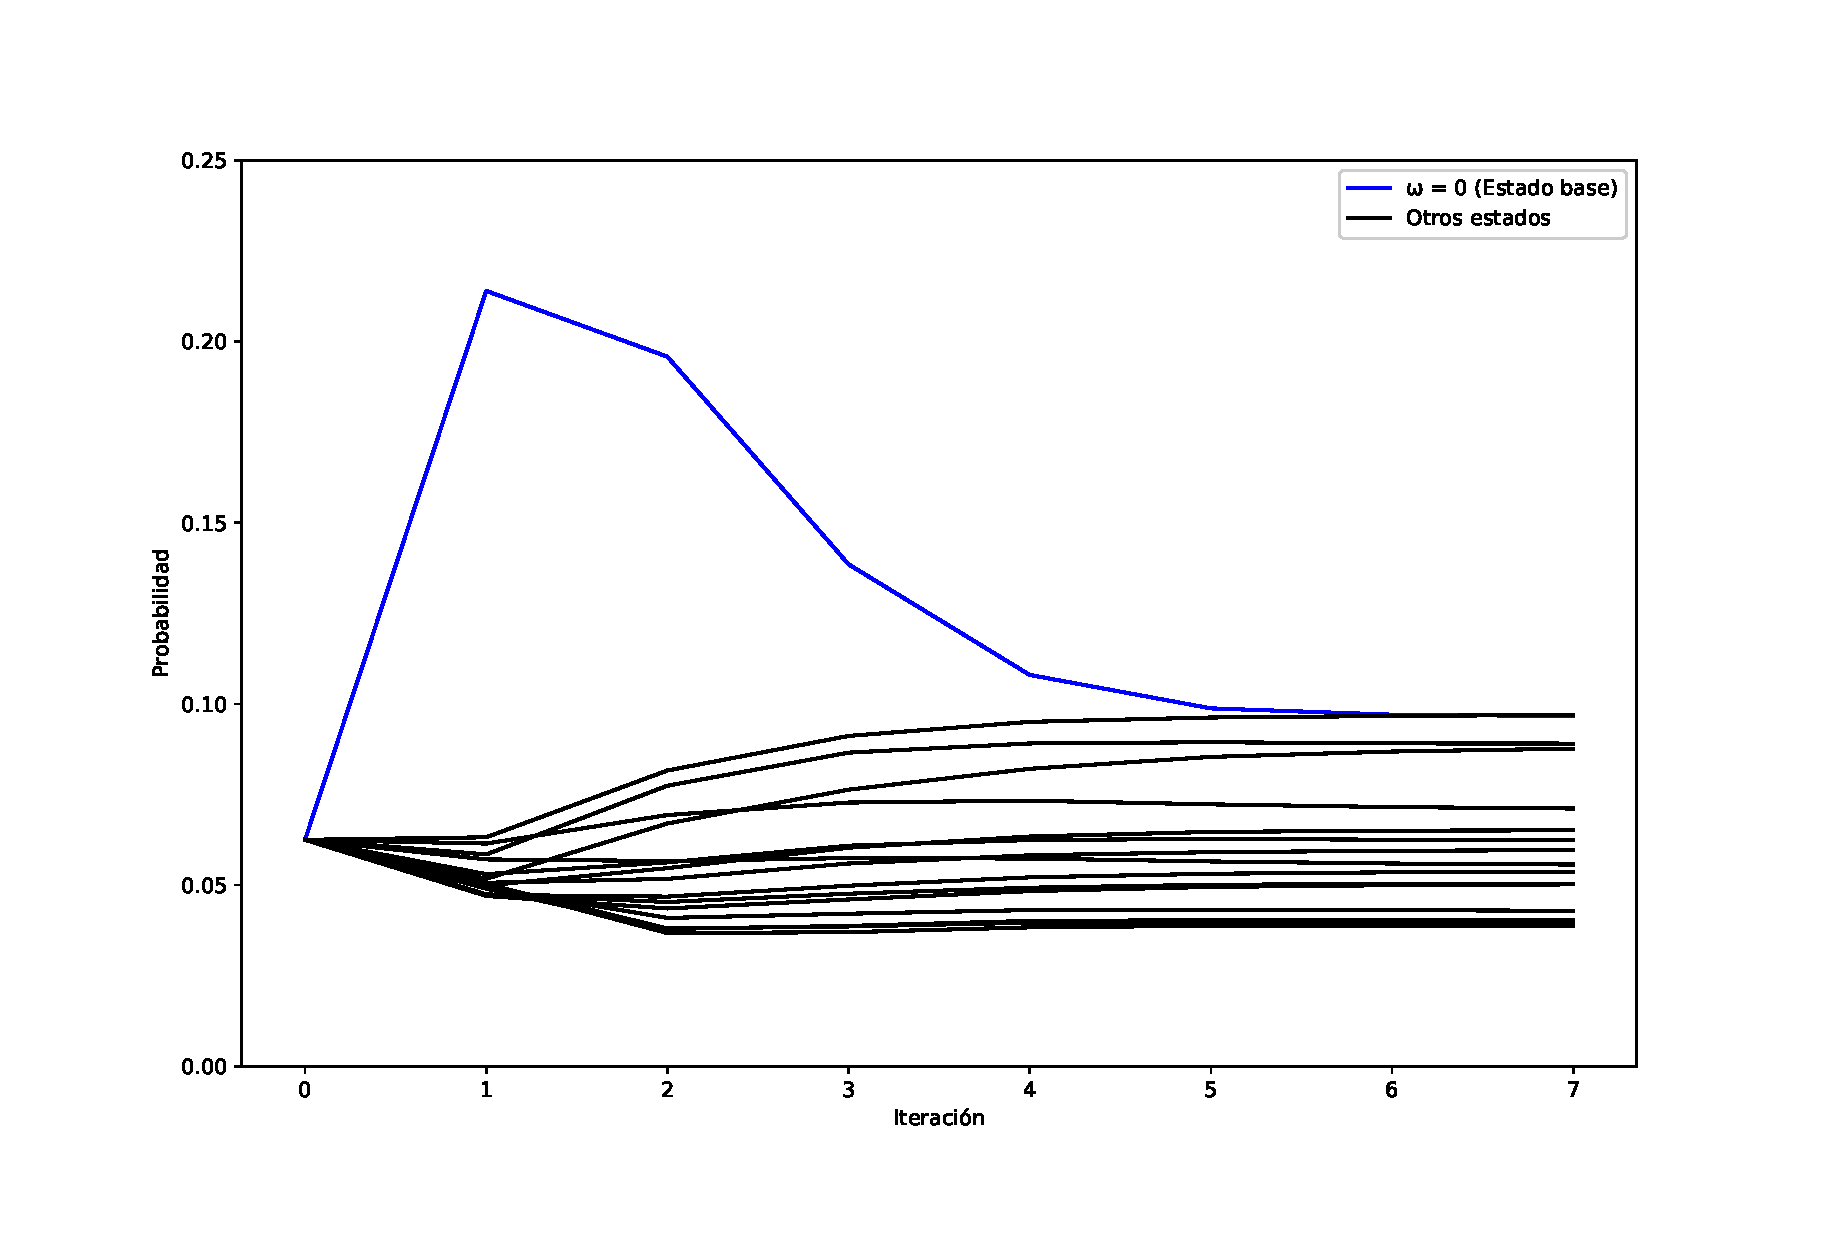
\includegraphics[width=0.99\linewidth]{img/grover0000loss.eps}
        \caption{Algoritmo de Grover con relajación. $\mathcal{W} = \{0\} = \{0000_2\}$}
    \end{figure}

\end{frame}

\begin{frame}
    \frametitle{Simulaciones del algoritmo de Grover}

    \begin{figure}[H]
        \centering
        \includegraphics[width=0.99\linewidth]{img/groverallloss.eps}
        \caption{$\omega = 15$}
        \caption{Algoritmo de Grover con relajación. $\mathcal{W} = \{15\} = \{1111_2\}$}
    \end{figure}

\end{frame}

\begin{frame}
    \frametitle{Simulaciones del algoritmo de Grover}
    \begin{figure}[H]
        \centering
        \includegraphics[width=0.9\linewidth]{img/grover2M.eps}
        \caption{Wolfram Mathematica: Algoritmo de amplificación de amplitud sin relajación, $\mathcal{W} = \{9, 13\}$}
    \end{figure}
\end{frame}

\begin{frame}
    \frametitle{Simulaciones del algoritmo de Grover}
    \vspace{-0.5cm}
    \begin{figure}[H]
        \centering
        \includegraphics[width=0.9\linewidth]{img/grover2lossless.eps}
        \caption{Python: Algoritmo de amplificación de amplitud sin relajación, $\mathcal{W} = \{9, 13\}$}
    \end{figure}

\end{frame}

\begin{frame}
    \frametitle{Simulaciones del algoritmo de Grover}
    \begin{figure}[H]
        \centering
        \includegraphics[width=0.99\linewidth]{img/grover2loss.eps}
        \caption{Algoritmo de amplificación de amplitud con relajación, $\mathcal{W} = \{9, 13\}$}
    \end{figure}
\end{frame}

\begin{frame}
    \frametitle{Simulaciones del algoritmo de Grover}
    \begin{figure}[H]
        \centering
        \includegraphics[width=0.9\linewidth]{img/grover3M.eps}
        \caption{Wolfram Mathematica: Algoritmo de amplificación de amplitud sin relajación, $\mathcal{W} = \{4, 5, 12, 13\} = \{0100_2, 0101_2, 1100_2, 1101_2\}$}
    \end{figure}
\end{frame}

\begin{frame}
    \frametitle{Simulaciones del algoritmo de Grover}
    \begin{figure}[H]
        \centering
        \includegraphics[width=0.9\linewidth]{img/grover3lossless.eps}
        \caption{Python: Algoritmo de amplificación de amplitud sin relajación, $\mathcal{W} = \{4, 5, 12, 13\} = \{0100_2, 0101_2, 1100_2, 1101_2\}$}
    \end{figure}

\end{frame}

\begin{frame}
    \frametitle{Simulaciones del algoritmo de Grover}
    \vspace{-0.5cm}
    \begin{figure}[H]
        \centering
        \includegraphics[width=0.99\linewidth]{img/grover3loss.eps}
        \caption{Algoritmo de amplificación de amplitud con relajación, $\mathcal{W} = \{4, 5, 12, 13\}$}
    \end{figure}

\end{frame}

\section{Algoritmo de Shor}

\begin{frame}
    \frametitle{Algoritmo de Shor}

    \justify
    El algoritmo de Shor es un algoritmo cuántico de factorización de enteros. Dado un entero $N=p \times q$, donde $p$ y $q$ son primos, el algoritmo de Shor encuentra $p$ y $q$ en $O((\log(N))^3)$ pasos, publicado en 1997 por Peter Shor \cite{Shor_1999}. El algoritmo clásico más eficiente para factorizar enteros es la cibra general del cuerpo de números y funciona con una complejidad heurística de $O(e^{(\sqrt[3]{\frac{64}{9}}+o(1))(\ln(N))^{\frac{1}{3}}(\ln(\ln(N)))^{\frac{2}{3}}})$. Por su capacidad de factorizar números semiprimos, el algoritmo de Shor es capaz de violar el cifrado RSA \cite{Bernstein_2017, Grosshans_2015} y el protocolo Diffie-Hellman de intercambio de llaves, sobre los cuáles se basa virtualmente toda la criptografía actual.
    \vspace{0.5cm}

    \justify
    El algoritmo de Shor está basado en el algoritmo de estimación de orden, el cuál es una aplicación del algoritmo de estimación de fase \cite{Nielsen_2009}. Éste último permite encontrar la fase $\phi$ del autovalor $e^{i \phi}$ asociado a algún autoestado $\ket{u}$ de un operador unitario U. El algoritmo de estimación de orden utiliza esta estimación para hallar el orden $r>0$ tal que $a^r \equiv 1 \mod m$, a partir del operador unitario de multiplicación modular.

\end{frame}

\begin{frame}
    \frametitle{Transformada cuántica de Fourier}

    \justify
    Esta transformada es equivalente a la transformada discreta de Fourier, sólo que a cada frecuencia se le asigna un ket. Cuando un estado tiene una distribución periódica, esta transformada sirve para hallar el período de tal distribución.

    La ecuación y el circuito de la transformada inversa de Fourier son los siguientes:

    \begin{equation}
        QFT^\dagger = \frac{1}{\sqrt{N}} \sum_x \sum_k e^{-2 \pi i k x / N} \ketbra{x}{k}
    \end{equation}

    \[\Qcircuit @C=1.4em @R=1.8em {
    \lstick{\ket{k_1}} & \qswap      & \qw      & \qw                   & \qw      & \gate{P_{-2 \pi/2^2}} & \gate{P_{-2 \pi/2^3}} & \gate{H} & \qw \\
    \lstick{\ket{k_2}} & \qw \qwx    & \qw      & \gate{P_{-2 \pi/2^2}} & \gate{H} & \ctrl{-1}             & \qw                   & \qw      & \qw \\
    \lstick{\ket{k_3}} & \qswap \qwx & \gate{H} & \ctrl{-1}             & \qw      & \qw                   & \ctrl{-2}             & \qw      & \qw \\
    } 
    \]

\end{frame}

\begin{frame}
    \frametitle{Estimación de fase y de orden}

    \justify
    El algoritmo de estimación de fase sirve para hallar los autovalores de un operador unitario $U$. Cuando este operador es el operador de multiplicación modular $U_{a, N} \ket{x} = \ket{a x \mod N}$ y el estado de entrada es $\ket{u} = \ket{1}$, el algoritmo sirve para estimar el orden de $a^x \mod N$.

\[\Qcircuit @C=1.4em @R=1.8em {
\lstick{\ket{0}^{\otimes K}}& {/^K}\qw & \gate{H^{\otimes K}} & \ctrl{1}   & \gate{QFT^\dagger} & \meter & \cw \\
\lstick{\ket{u} \quad}      & {/^L}\qw & \qw                  & \gate{U^j} & \qw                & \qw    & \qw \\
} 
\]

\end{frame}

\begin{frame}
    \frametitle{Algoritmo de Shor}

    \begin{enumerate}
        \item Si es $N$ es par o un cuadrado perfecto, se conoce una factorización. Fin del algoritmo.
        \item Elegir un número aleatorio $a < N$.
        \item Si $GCD(a,N) \neq 1$, entonces este número es un factor no trivial de N y se ha hallado una factorización. Fin del algoritmo.
        \item Si $a$ es par, volver al paso 3.
        \item Si no, usar el algoritmo de estimación de orden para hallar el período $r$ de $f(x) = a^x \mod N$.
        \item Si r es impar, volver al paso 3.
        \item Si $a^{r} \not\equiv 1 \mod N$, ir al paso 3.
        \item Si $a^{r/2} \equiv -1 \mod N$, ir al paso 3.
        \item Finalmente, $GCD(a^{r/2} + 1, N)$ y $GCD(a^{r/2} - 1, N)$ son factores de $N$. Fin del algoritmo.
    \end{enumerate}

\end{frame}

\begin{frame}
    \frametitle{Simulaciones del algoritmo de Shor}

\begin{figure}[H]
    \centering
    \begin{subfigure}[m]{0.47\textwidth}
        \centering
        \includegraphics[width=0.95\linewidth]{img/ShorM15.png}
        \caption{Wolfram Mathematica}
    \end{subfigure}
    \begin{subfigure}[m]{0.47\textwidth}
        \centering
        \includegraphics[width=0.95\linewidth]{img/shorlossless.png}
        \caption{Python}
    \end{subfigure}
    \caption{Estimación de fase del algoritmo de Shor sin pérdidas para el número 15}
    \label{fig:shor15}
\end{figure}

\end{frame}

\begin{frame}
    \frametitle{Simulaciones del algoritmo de Shor}

\begin{figure}[H]
    \centering
    \begin{subfigure}[m]{0.47\textwidth}
        \centering
        \includegraphics[width=0.95\linewidth]{img/ShorM8.png}
        \caption{Wolfram Mathematica}
    \end{subfigure}
    \begin{subfigure}[m]{0.47\textwidth}
        \centering
        \includegraphics[width=0.95\linewidth]{img/shor2lossless.png}
        \caption{Python}
    \end{subfigure}
    \caption{Estimación de fase del algoritmo de Shor sin pérdidas para el número 8}
    \label{fig:shor8}
\end{figure}

\end{frame}

\section{PageRank}

\begin{frame}
    \frametitle{PageRank}

    El algoritmo de PageRank fue desarrollado en 1996 en la Universidad de Stanford por Larry Page y Sergey Brin \cite{Brin_1998}, los cuales fueron los fundadores de Google.
    \vspace{0.5cm}

    Este algoritmo se basa en la idea de que sitios web importantes tienen muchos vínculos que apuntan hacia ellos, lo que conduce a pensar en la web como una red ponderada orientada. Existen muchos otros algoritmos, algunos más eficientes, pero la importancia de PageRank se sustenta en el poder económico de Google.
    \vspace{0.5cm}

    El primer paso de este algoritmo es construir la matriz de adyacencia ponderada del grafo a procesar

    \begin{equation}
        E_{ij} \equiv \begin{cases}
        \frac{1}{\mathrm{outdeg}(P_j)} & \text{si el nodo } P_j \text{ tiene un hipervínculo a } P_i \\
        0 & \text{en otro caso}
        \end{cases}
    \end{equation}
\end{frame}

\begin{frame}
    \frametitle{PageRank}

    Para considerar los casos en los que se entra directamente a página por su URL, en lugar de un hipervínculo, se agrega el término $\mathds{I}$

    \begin{equation}
        G \equiv \alpha E + \frac{1-\alpha}{N} \mathds{I} \quad \text{ (Matriz de Google)}
    \end{equation}

    $\mathds{I}$ es una matriz en la cual todas las entradas están establecidas en 1, y N el número de nodos. El PageRank del grafo está dado por el vector al que converge la siguiente sucesión, para cualquier vector $I^0$ inicial

    \begin{equation}
        I^k = G I^{k-1}
    \end{equation}

    \begin{figure}[H]
    \begin{center}
    \begin{tikzpicture}[->,>=stealth',shorten >=1pt,thick]
    \tikzset{VertexStyle/.style = {draw,circle,thick,
                                   minimum size=0.5cm,
                                   font=\bfseries},thick} 
    \Vertex[a = 90, d = 2]{1}  \Vertex[a = 162, d = 2]{2}
    \Vertex[a = 234, d = 2]{3} \Vertex[a = 306, d = 2]{4}
    \Vertex[a = 18, d = 2]{5}
    \Edge[label=$1$](2)(1)
    \Edge[label=$1$](1)(5)
    \Edge[label=$\frac{1}{2}$](3)(1)
    \Edge[label=$\frac{1}{2}$](3)(4)
    \Edge[label=$1$](4)(5)
    \tikzset{EdgeStyle/.style = {->, bend left}}
    \Edge[label=$1$](1)(3)
    \end{tikzpicture} 
\end{center}\end{figure}\end{frame}


\begin{frame}
    \frametitle{PageRank}

    Transformación de un grafo al crear la matriz de Google con $\alpha = \frac{1}{2}$
    \vspace{-0.25cm}

    \begin{figure}[H]
    \begin{center}
    \begin{tikzpicture}[->,>=stealth',shorten >=1pt,thick]
    \tikzset{VertexStyle/.style = {draw,circle,thick,
                                   minimum size=0.5cm,
                                   font=\bfseries},thick} 
    \Vertex[a = 90, d = 2.75]{1}  \Vertex[a = 162, d = 2.75]{2}
    \Vertex[a = 234, d = 2.75]{3} \Vertex[a = 306, d = 2.75]{4}
    \Vertex[a = 18, d = 2.75]{5}
    \Edge[label=$\frac{1}{10}$](5)(4)
    \Edge[label=$\frac{1}{10}$](4)(3)
    \Edge[label=$\frac{1}{10}$](3)(2)
    \Edge[label=$\frac{3}{5}$](2)(1)
    \Edge[label=$\frac{3}{5}$](1)(5)
    \Edge[label=$\frac{1}{10}$](1)(4)
    \Edge[label=$\frac{1}{10}$](4)(2)
    \Edge[label=$\frac{1}{10}$](2)(5)
    \Edge[label=$\frac{1}{10}$](5)(3)
    \Edge[label=$\frac{7}{20}$](3)(1)
    \Loop[dist=1cm,dir=NO,label=$\frac{1}{10}$,labelstyle=above](1)  
    \Loop[dist=1cm,dir=NOWE,label=$\frac{1}{10}$,labelstyle=above left](2)  
    \Loop[dist=1cm,dir=SOWE,label=$\frac{1}{10}$,labelstyle=below left](3)  
    \Loop[dist=1cm,dir=SOEA,label=$\frac{1}{10}$,labelstyle=below right](4)  
    \Loop[dist=1cm,dir=NOEA,label=$\frac{1}{10}$,labelstyle=above right](5)  
    \tikzset{EdgeStyle/.style = {->, bend right}}
    \Edge[label=$\frac{1}{10}$,labelstyle=above left](1)(2)
    \Edge[label=$\frac{1}{10}$,labelstyle=below left](2)(3)
    \Edge[label=$\frac{7}{20}$,labelstyle=below](3)(4)
    \Edge[label=$\frac{3}{5}$,labelstyle=below right](4)(5)
    \Edge[label=$\frac{1}{10}$,labelstyle=above right](5)(1)
    \Edge[label=$\frac{3}{5}$](1)(3)
    \Edge[label=$\frac{1}{10}$](3)(5)
    \Edge[label=$\frac{1}{10}$](5)(2)
    \Edge[label=$\frac{1}{10}$](2)(4)
    \Edge[label=$\frac{1}{10}$](4)(1)
    \end{tikzpicture} 
    \end{center}
    \end{figure}

\end{frame}

\begin{frame}
    \frametitle{Caminatas cuánticas}

    El método que parecería trivial, para cuantizar las caminatas aleatorias, de asignar un ket a cada nodo, no es realizable.

    \begin{figure}[H]
    \begin{tikzpicture}[,>=stealth',shorten >=1pt,thick]
    \tikzset{VertexStyle/.style = {draw,circle,thick,
                                   minimum size=1cm,
                                   font=\bfseries},thick} 
    \Vertex[x = -3, y = 0]{-2}  \Vertex[x = -1.5, y = 0]{-1}
    \Vertex[x = 0, y = 0]{0} \Vertex[x = 1.5, y = 0]{1}
    \Vertex[x = 3, y = 0]{2}
    \Edges(-2,-1,0,1,2)
    \end{tikzpicture}
    \end{figure}

    Al hacer esto, aparecen operadores no unitarios, los cuales no son realizables con compuertas cuánticas.

    \begin{figure}[H]
    \begin{tikzpicture}[,>=stealth',shorten >=1pt,thick]
    \tikzset{VertexStyle/.style = {draw,circle,thick,
                                   minimum size=1cm,
                                   font=\scriptsize\bfseries},thick} 
    \Vertex[x = -3, y = 0, L = $\ket{-2}$]{-2}  \Vertex[x = -1.5, y = 0, L = $\ket{-1}$]{-1}
    \Vertex[x = 0, y = 0, L = $\ket{0}$]{0} \Vertex[x = 1.5, y = 0, L = $\ket{1}$]{1}
    \Vertex[x = 3, y = 0, L = $\ket{2}$]{2}
    \Edges(-2,-1,0,1,2)
    \end{tikzpicture}
    \end{figure}

\end{frame}

\begin{frame}
    \frametitle{Caminatas cuánticas de Szegedy}

    \justify
    Para solucionar esto, Szegedy propuso duplicar los nodos del grafo y construir un grafo bipartito a partir de él. Un grafo bipartito es aquel donde los nodos se pueden separar en dos particiones y no hay vínculos entre nodos de la misma partición.

    \begin{figure}[h]
    \begin{tikzpicture}[->,>=stealth',shorten >=1pt,thick]
    \SetGraphUnit{2} 
    \tikzset{VertexStyle/.style = {draw,circle,thick,
                                   minimum size=0.5cm,
                                   font=\bfseries},thick} 
    \Vertex{1} \SOWE(1){2} \SOEA(2){3} \SOEA(1){4} 
    \Edges(1,2,3) \Edge(1)(4)

    \tikzset{EdgeStyle/.style = {->, bend left}}
    \Edge(3)(2)
    % it's possible with \Edge but Tikz's syntax is allowed too.
    \end{tikzpicture} 
\end{figure}\end{frame}

\begin{frame}
    \frametitle{Caminatas cuánticas de Szegedy}

    \justify
    A cada nodo se le asigna un estado de la siguiente forma

    \begin{minipage}{0.45\linewidth}
    \begin{align*}
    \ket{\psi_i} &= \ket{i}_1 \otimes \sum\limits_j \sqrt{p_{j i}} \ket{j}_2 \\
    A &= \sum\limits_i \ketbra{\psi_i}{\psi_i}
    \end{align*}
    \end{minipage}
    \begin{minipage}{0.45\linewidth}
    \begin{align*}
    \ket{\psi_i} &= \sum\limits_i \sqrt{p_{i j}} \ket{i}_1 \otimes \ket{i}_2 \\
    B &= \sum\limits_j \ketbra{\phi_j}{\phi_j} .
    \end{align*}
    \end{minipage}

    \begin{figure}[h]
    \begin{tabular}{c c}
    \begin{tikzpicture}[->,>=stealth',shorten >=1pt,thick]
    \tikzset{VertexStyle/.style = {draw,circle,thick,
                                   minimum size=0.5cm,
                                   font=\bfseries},thick} 
    \Vertex[x = 0, y = 0]{1a} \Vertex[x = 0, y = -1]{2a}
    \Vertex[x = 0, y = -2]{3a}\Vertex[x = 0, y = -3]{4a}
    \Vertex[x = 3, y = 0]{1b} \Vertex[x = 3, y = -1]{2b}
    \Vertex[x = 3, y = -2]{3b}\Vertex[x = 3, y = -3]{4b}
    \Edge(1a)(2b)	\Edge(1a)(4b)	\Edge(2a)(3b)
    \Edge(3a)(2b)
    \end{tikzpicture}
    &
    \begin{tikzpicture}[->,>=stealth',shorten >=1pt,thick]
    \tikzset{VertexStyle/.style = {draw,circle,thick,
                                   minimum size=0.5cm,
                                   font=\bfseries},thick} 
    \Vertex[x = 0, y = 0]{1a} \Vertex[x = 0, y = -1]{2a}
    \Vertex[x = 0, y = -2]{3a}\Vertex[x = 0, y = -3]{4a}
    \Vertex[x = 3, y = 0]{1b} \Vertex[x = 3, y = -1]{2b}
    \Vertex[x = 3, y = -2]{3b}\Vertex[x = 3, y = -3]{4b}
    \Edge(2b)(1a)	\Edge(4b)(1a)	\Edge(3b)(2a)
    \Edge(2b)(3a)
    \end{tikzpicture}
    \end{tabular}
    \end{figure}

    \justify
    De esta manera, el operador que genera la caminata es $U = (\mathds{1} - 2 B)(\mathds{1} - 2 A)$

\end{frame}

\begin{frame}
    \frametitle{PageRank cuántico}

    El PageRank cuántico instantaneo de cada nodo en el paso $m$ es la probabilidad de encontrar encontrar al caminante en ese nodo, midiendo la segunda partición y comenzando la caminata con el estado inicial $\ket{\psi_0}$

    \begin{equation}
        I_q(P_i,m) =  Tr((\mathds{1} \otimes \ketbra{i}{i}) U^m \ketbra{\psi_0} U^{\dagger m})
    \end{equation}

    \begin{equation}
        \ket{\psi_0} = \frac{1}{\sqrt{N}} \sum\limits_i \ket{\psi_i}
    \end{equation}

    Sin embargo, este valor no converge, sino que oscila. Así que tomamos, como medida de centralidad, el PageRank cuántico promedio, el cual sí converge.

    \begin{equation}
        \langle I_q(P_i) \rangle = \frac{1}{M} \sum\limits_{m=0}^{M-1} I_q(P_i,m)
    \end{equation}

\end{frame}

\begin{frame}
    \frametitle{Circuitos de Loke}

    \justify
    Loke desarrolló un método para construir los circuitos de las caminatas cuánticas de Szegedy, diagonalizando el operador $U$ de la caminata. Primero, dividimos el grafo en subgrafos cíclicos. El operador $T$ convierte los estados de todos los nodos de cada subgrafo en el de algún nodo de referencia del mismo subgrafo. El operador $K_b^\dagger$ convierte los estados de los nodos de referencia en un estado de la base computacional para el cuál podamos construir el operador de reflexión.

    \begin{figure}[H]
    \[\Qcircuit @C=1.4em @R=1.8em {
            \lstick{\text{Registro 1}}& {/}\qw & \ctrl{1}   & \ctrl{1}           & \qw      & \ctrl{1}   & \ctrl{1}           & \qswap     & \qw \\
            \lstick{\text{Registro 2}}& {/}\qw & \gate{T_i} & \gate{K_b^\dagger} & \gate{D} & \gate{K_b} & \gate{T_i^\dagger} & \qswap\qwx & \qw \\
    & & & & \rstick{\hspace{-13pt} 2 \text{ veces}}
    \gategroup{2}{3}{2}{8}{1.5em}{_\}}
    } 
    \]
    \caption[Circuito de Loke \cite{loke} para las caminatas cuánticas de Szegedy]{Circuito de Loke para las caminatas cuánticas de Szegedy}
    \label{fig:lokecircuit}
    \end{figure}

    Cada uno de los registros corresponde a una de las particiones del grafo bipartito.

\end{frame}

\begin{frame}
    \frametitle{Circuitos de Loke}

    Los operadores $T_i$ se pueden construir de manera general con operadores de permutación $T$

    \begin{figure}[H]
    \[\Qcircuit @C=1.4em @R=1.8em {
            & \targ     & \qw      & \qw \\
            & \ctrl{-1} & \gate{X} & \qw \\
    } 
    \]
    \caption[Operador de permutación]{Operador de permutación $T$}
    \label{fig:T}
    \end{figure}

    Sin embargo, Loke no presenta ninguna manera de construir los operadores $K_b$. Sólo presenta algunos casos particulares como ejemplos. Como parte de este trabajo se ha desarrollado un método para construir estos operadores par cualquier grafo de 4 nodos, a partir de los coeficientes $\sqrt{G_i}$ del estado inicial $\ket{\psi_0}$ de la caminata.

\end{frame}

\begin{frame}
    \frametitle{Circuitos de Loke}

\begin{figure}[H]
\[\Qcircuit @C=1.4em @R=1.8em {
& \gate{Ry(\theta_{00})} & \ctrlo{1}               & \ctrl{1}               & \qw \\
& \qw                    & \gate{Ry(\theta_{10})}  & \gate{Ry(\theta_{11})} & \qw \\
} \]
\caption{Circuito de $K_i$}
\end{figure}

\begin{align}
    \theta_{00} &= 2 \cos^{-1}\left(\sqrt{G_1 + G_2}\right) \\
    \theta_{10} &= 2 \cos^{-1}\left(\sqrt{\frac{G_1}{G_1 + G_2}}\right) \\
    \theta_{11} &= 2 \cos^{-1}\left(\sqrt{\frac{G_3}{1 - (G_1 + G_2)}}\right) .
\end{align}

\end{frame}

\begin{frame}
    \frametitle{Simulaciones del algoritmo de PageRank cuántico}


\begin{figure}[H]
    \centering
    \begin{tikzpicture}[->,>=stealth',shorten >=1pt,thick]
    \SetGraphUnit{2} 
    \tikzset{VertexStyle/.style = {draw,circle,thick,
                                   minimum size=0.5cm,
                                   font=\bfseries},thick} 
    \Vertex{1} \NO(1){2} \SOEA(1){3} \SOWE(1){4} 
    \Edge(1)(2)
    \Edge(1)(3)
    \Edge(1)(4)
    
    \tikzset{EdgeStyle/.style = {->, bend left}}
    \Edge(2)(1)
    \Edge(3)(1)
    \Edge(4)(1)
    \end{tikzpicture} 
    \caption[Grafo estrella]{Grafo estrella}
    \label{fig:star}
\end{figure}

\end{frame}

\begin{frame}
    \frametitle{Simulaciones del algoritmo de PageRank cuántico}

\begin{equation}
    A =
    \begin{pmatrix}
        0 & 1 & 1 & 1 \\
        1 & 0 & 0 & 0 \\
        1 & 0 & 0 & 0 \\
        1 & 0 & 0 & 0
    \end{pmatrix}
\end{equation}

\begin{equation}
    E = 
    \begin{pmatrix}
        0 & 1 & 1 & 1 \\
        \frac{1}{3} & 0 & 0 & 0 \\
        \frac{1}{3} & 0 & 0 & 0 \\
        \frac{1}{3} & 0 & 0 & 0
    \end{pmatrix}
\end{equation}

\begin{equation}
    G =
    \begin{pmatrix}
        \frac{3}{80} & \frac{71}{80} & \frac{71}{80} & \frac{71}{80} \\
        \frac{77}{240} & \frac{3}{80} & \frac{3}{80} & \frac{3}{80} \\
        \frac{77}{240} & \frac{3}{80} & \frac{3}{80} & \frac{3}{80} \\
        \frac{77}{240} & \frac{3}{80} & \frac{3}{80} & \frac{3}{80}
    \end{pmatrix}
\end{equation}

\end{frame}

\begin{frame}
    \frametitle{Simulaciones del algoritmo de PageRank cuántico}

\begin{figure}[H]
    \centering
    \includegraphics[width=0.9\linewidth]{img/star-inst-M.eps}
    \caption{Wolfram Mathematica: PageRank cuántico instantáneo del grafo estrella sin pérdidas}
\end{figure}

\end{frame}

\begin{frame}
    \frametitle{Simulaciones del algoritmo de PageRank cuántico}

\begin{figure}[H]
    \centering
    \includegraphics[width=0.9\linewidth]{img/star-inst-lossless.eps}
    \caption{Python: PageRank cuántico instantáneo del grafo estrella sin pérdidas}
\end{figure}

\end{frame}

\begin{frame}
    \frametitle{Simulaciones del algoritmo de PageRank cuántico}

    \begin{figure}[H]
        \centering
        \includegraphics[width=0.9\linewidth]{img/star-mean-M.eps}
        \caption{Wolfram Mathematica: PageRank cuántico promedio del grafo estrella sin pérdidas}
    \end{figure}

\end{frame}

\begin{frame}
    \frametitle{Simulaciones del algoritmo de PageRank cuántico}

    \begin{figure}[H]
        \centering
        \includegraphics[width=0.9\linewidth]{img/star-mean-lossless.eps}
        \caption{PageRank cuántico promedio del grafo estrella sin pérdidas}
    \end{figure}

\end{frame}

\begin{frame}
    \frametitle{Simulaciones del algoritmo de PageRank cuántico}

    \begin{figure}[H]
        \centering
        \includegraphics[width=0.9\linewidth]{img/star-inst-lossy.eps}
        \caption{PageRank cuántico instantaneo del grafo estrella con pérdidas}
    \end{figure}

\end{frame}





\begin{frame}
    \frametitle{Simulaciones del algoritmo de PageRank cuántico}


\begin{figure}[H]
    \centering
    \begin{tikzpicture}[->,>=stealth',shorten >=1pt,thick]
    \SetGraphUnit{2} 
    \tikzset{VertexStyle/.style = {draw,circle,thick,
                                   minimum size=0.5cm,
                                   font=\bfseries},thick} 
    \Vertex{4} \NO(4){1} \SOEA(4){2} \SOWE(4){3} 
    \Edge(1)(4)
    \Edge(2)(4)
    \Edge(3)(4)
    \Edges(3,2,1,3)
    \tikzset{EdgeStyle/.style = {->, bend left}}
    \Edges(1,2,3,1)
    \end{tikzpicture} 
    \caption[Grafo corona]{Grafo corona}
    \label{fig:crown}
\end{figure}

\end{frame}

\begin{frame}
    \frametitle{Simulaciones del algoritmo de PageRank cuántico}

\begin{equation}
    A =
    \begin{pmatrix}
        0 & 1 & 1 & 0 \\
        1 & 0 & 1 & 0 \\
        1 & 1 & 0 & 0 \\
        1 & 1 & 1 & 0 \\
    \end{pmatrix}
\end{equation}

\begin{equation}
    E =
    \begin{pmatrix}
        0 & \frac{1}{3} & \frac{1}{3} & \frac{1}{4} \\
        \frac{1}{3} & 0 & \frac{1}{3} & \frac{1}{4} \\
        \frac{1}{3} & \frac{1}{3} & 0 & \frac{1}{4} \\
        \frac{1}{3} & \frac{1}{3} & \frac{1}{3} & \frac{1}{4} \\
    \end{pmatrix}
\end{equation}

\begin{equation}
    G =
    \begin{pmatrix}
        \frac{3}{80} & \frac{77}{240} & \frac{77}{240} & \frac{1}{4} \\
        \frac{77}{240} & \frac{3}{80} & \frac{77}{240} & \frac{1}{4} \\
        \frac{77}{240} & \frac{77}{240} & \frac{3}{80} & \frac{1}{4} \\
        \frac{77}{240} & \frac{77}{240} & \frac{77}{240} & \frac{1}{4} \\
    \end{pmatrix}
\end{equation}

\end{frame}

\begin{frame}
    \frametitle{Simulaciones del algoritmo de PageRank cuántico}

    \begin{figure}[H]
        \centering
        \includegraphics[width=0.9\linewidth]{img/crown-inst-M.eps}
        \caption{Wolfram Mathematica: PageRank cuántico instantáneo del grafo corona sin pérdidas}
    \end{figure}

\end{frame}

\begin{frame}
    \frametitle{Simulaciones del algoritmo de PageRank cuántico}

    \begin{figure}[H]
        \centering
        \includegraphics[width=0.9\linewidth]{img/crown-inst-lossless.eps}
        \caption{Python: PageRank cuántico instantáneo del grafo corona sin pérdidas}
\end{figure}

\end{frame}

\begin{frame}
    \frametitle{Simulaciones del algoritmo de PageRank cuántico}

    \begin{figure}[H]
        \centering
        \includegraphics[width=0.9\linewidth]{img/crown-mean-M.eps}
        \caption{Wolfram Mathematica: PageRank cuántico promedio del grafo corona sin pérdidas}
    \end{figure}

\end{frame}

\begin{frame}
    \frametitle{Simulaciones del algoritmo de PageRank cuántico}

    \begin{figure}[H]
        \centering
        \includegraphics[width=0.9\linewidth]{img/crown-mean-lossless.eps}
        \caption{Python: PageRank cuántico promedio del grafo corona sin pérdidas}
    \end{figure}

\end{frame}

\begin{frame}
    \frametitle{Simulaciones del algoritmo de PageRank cuántico}

    \begin{figure}[H]
        \centering
        \includegraphics[width=0.9\linewidth]{img/crown-inst-lossy.eps}
        \caption{PageRank cuántico instantaneo del grafo aleatorio con pérdidas}
    \end{figure}

\end{frame}




\begin{frame}
    \frametitle{Simulaciones del algoritmo de PageRank cuántico}

    \begin{figure}[H]
        \centering
        \begin{tikzpicture}[->,>=stealth',shorten >=1pt,thick]
        \SetGraphUnit{2} 
        \tikzset{VertexStyle/.style = {draw,circle,thick,
                                       minimum size=0.5cm,
                                       font=\bfseries},thick} 
        \Vertex{1} \SOWE(1){2} \SOEA(1){3} \SO(2){4} 
        \Edge(1)(2)
        \Edge(1)(3)
        \Edge(2)(4)
        \end{tikzpicture} 
        \caption[Grafo árbol]{Grafo árbol}
        \label{fig:tree}
    \end{figure}

\end{frame}

\begin{frame}
    \frametitle{Simulaciones del algoritmo de PageRank cuántico}

\begin{equation}
    A = 
    \begin{pmatrix}
        0 & 0 & 0 & 0 \\
        1 & 0 & 0 & 0 \\
        1 & 0 & 0 & 0 \\
        0 & 1 & 0 & 0 \\
    \end{pmatrix}
\end{equation}

\begin{equation}
    E =
    \begin{pmatrix}
        0 & 0 & \frac{1}{4} & \frac{1}{4} \\
        \frac{1}{2} & 0 & \frac{1}{4} & \frac{1}{4} \\
        \frac{1}{2} & 0 & \frac{1}{4} & \frac{1}{4} \\
        0 & 1 & \frac{1}{4} & \frac{1}{4} \\
    \end{pmatrix}
\end{equation}

\begin{equation}
    G =
    \begin{pmatrix}
        \frac{3}{80} & \frac{3}{80} & \frac{1}{4} & \frac{1}{4} \\
        \frac{37}{80} & \frac{3}{80} & \frac{1}{4} & \frac{1}{4} \\
        \frac{37}{80} & \frac{3}{80} & \frac{1}{4} & \frac{1}{4} \\
        \frac{3}{80} & \frac{71}{80} & \frac{1}{4} & \frac{1}{4} \\
    \end{pmatrix}
\end{equation}

\end{frame}

\begin{frame}
    \frametitle{Simulaciones del algoritmo de PageRank cuántico}

    \begin{figure}[H]
        \centering
        \includegraphics[width=0.9\linewidth]{img/tree-inst-M.eps}
        \caption{Wolfram Mathematica: PageRank cuántico instantáneo del grafo árbol sin pérdidas}
    \end{figure}

\end{frame}

\begin{frame}
    \frametitle{Simulaciones del algoritmo de PageRank cuántico}

    \begin{figure}[H]
        \centering
        \includegraphics[width=0.9\linewidth]{img/tree-inst-lossless.eps}
        \caption{Python: PageRank cuántico instantáneo del grafo árbol sin pérdidas}
    \end{figure}

\end{frame}

\begin{frame}
    \frametitle{Simulaciones del algoritmo de PageRank cuántico}

    \begin{figure}[H]
        \centering
        \includegraphics[width=0.9\linewidth]{img/tree-mean-M.eps}
        \caption{Wolfram Mathematica: PageRank cuántico promedio del grafo árbol sin pérdidas}
    \end{figure}

\end{frame}

\begin{frame}
    \frametitle{Simulaciones del algoritmo de PageRank cuántico}

    \begin{figure}[H]
        \centering
        \includegraphics[width=0.9\linewidth]{img/tree-mean-lossless.eps}
        \caption{Python: PageRank cuántico promedio del grafo árbol sin pérdidas}
\end{figure}

\end{frame}

    \begin{frame}
        \frametitle{Simulaciones del algoritmo de PageRank cuántico}

        \begin{figure}[H]
            \centering
            \includegraphics[width=0.9\linewidth]{img/tree-inst-lossy.eps}
            \caption{PageRank cuántico instantaneo del grafo árbol con pérdidas}
    \end{figure}

\end{frame}




\begin{frame}
    \frametitle{Simulaciones del algoritmo de PageRank cuántico}


    \begin{figure}[H]
        \centering
        \begin{tikzpicture}[->,>=stealth',shorten >=1pt,thick]
        \SetGraphUnit{2} 
        \tikzset{VertexStyle/.style = {draw,circle,thick,
                                       minimum size=0.5cm,
                                       font=\bfseries},thick} 
        \Vertex{1} \SOWE(1){2} \SOEA(1){3} \SOEA(2){4} 
        \Edge(1)(2)
        \Edge(1)(3)
        \Edge(1)(4)
        \Edge(2)(4)
        \Edge(3)(4)

        \tikzset{EdgeStyle/.style = {->, bend left}}
        \Edge(2)(1)
        \tikzset{EdgeStyle/.style = {->, bend right}}
        \Edge(4)(3)
        \end{tikzpicture} 
        \caption[Grafo aleatorio]{Grafo aleatorio}
        \label{fig:any}
    \end{figure}

\end{frame}

\begin{frame}
    \frametitle{Simulaciones del algoritmo de PageRank cuántico}

\begin{equation}
    A =
    \begin{pmatrix}
        0 & 1 & 0 & 0 \\
        1 & 0 & 0 & 0 \\
        1 & 0 & 0 & 1 \\
        1 & 1 & 1 & 0 \\
    \end{pmatrix}
\end{equation}

\begin{equation}
    E =
    \begin{pmatrix}
        0 & \frac{1}{2} & 0 & 0 \\
        \frac{1}{3} & 0 & 0 & 0 \\
        \frac{1}{3} & 0 & 0 & 1 \\
        \frac{1}{3} & \frac{1}{2} & 1 & 0 \\
    \end{pmatrix}
\end{equation}

\begin{equation}
    G =
    \begin{pmatrix}
        \frac{3}{80} & \frac{37}{80} & \frac{3}{80} & \frac{3}{80} \\
        \frac{77}{240} & \frac{3}{80} & \frac{3}{80} & \frac{3}{80} \\
        \frac{77}{240} & \frac{3}{80} & \frac{3}{80} & \frac{71}{80} \\
        \frac{77}{240} & \frac{37}{80} & \frac{71}{80} & \frac{3}{80} \\
    \end{pmatrix}
\end{equation}

\end{frame}

\begin{frame}
    \frametitle{Simulaciones del algoritmo de PageRank cuántico}

    \begin{figure}[H]
        \centering
        \includegraphics[width=0.9\linewidth]{img/any-inst-M.eps}
        \caption{Wolfram Mathematica: PageRank cuántico instantáneo del grafo aleatorio sin pérdidas}
    \end{figure}

\end{frame}

\begin{frame}
    \frametitle{Simulaciones del algoritmo de PageRank cuántico}

    \begin{figure}[H]
        \centering
        \includegraphics[width=0.9\linewidth]{img/any-inst-lossless.eps}
        \caption{Python: PageRank cuántico instantáneo del grafo aleatorio sin pérdidas}
    \label{fig:instanylossless}
    \end{figure}

\end{frame}

\begin{frame}
    \frametitle{Simulaciones del algoritmo de PageRank cuántico}

    \begin{figure}[H]
        \centering
        \includegraphics[width=0.9\linewidth]{img/any-mean-M.eps}
        \caption{Wolfram Mathematica: PageRank cuántico promedio del grafo aleatorio sin pérdidas}
    \end{figure}

\end{frame}

\begin{frame}
    \frametitle{Simulaciones del algoritmo de PageRank cuántico}

    \begin{figure}[H]
        \centering
        \includegraphics[width=0.9\linewidth]{img/any-mean-lossless.eps}
        \caption{Python: PageRank cuántico promedio del grafo aleatorio sin pérdidas}
    \end{figure}

\end{frame}

\begin{frame}
    \frametitle{Simulaciones del algoritmo de PageRank cuántico}

    \begin{figure}[H]
            \centering
            \includegraphics[width=0.9\linewidth]{img/any-inst-lossy.eps}
            \caption{PageRank cuántico instantaneo del grafo aleatorio con pérdidas}
    \end{figure}

\end{frame}


\section{Conclusiones}

\begin{frame}
    \frametitle{Conclusiones}

    En el presente trabajo se ha:

    \begin{enumerate}
        \item Estudiado las bases de teoría de información cuántica y de superconductividad necesarias para entender la dinámica de los transmones.
        \item Construido la representación circuital cuántica de los AC de Grover, Shor y de Google Cuántico.
        \item Hallado las secuencias de pulsos que generan las compuertas necesarias para los algoritmos estudiados.
        \item Simulado en Mathematica, de forma algebraica, cada uno de los AC seleccionados y se ha simulado en Python la implementación de estos en transmones.
    \end{enumerate}

    Los resultados de las simulaciones del algoritmo de Grover y PageRank nos indican que para sistemas con tiempos de relajación del orden de $O(10^4 ns)$, los protocolos de corrección de errores cuánticos son una necesidad. Este es un resultado importante, pues el record actual de tiempo de vida de un qubit superconductor es inferior a 0.1ms, está en el mismo orden de magnitud que el del sistema simulado.

\end{frame}

\begin{frame}
    \frametitle{Conclusiones}

    Hasta donde tenemos conocimiento, ninguno de los siguientes aportes se encuentran en la literatura científica:

    \begin{enumerate}
        \item Una compuerta controlada de fase CP que permita eliminar las fases en las compuertas de negación con dos o más qubits de control, como la de Toffoli.
        \item Un conjunto de instrucciones cuánticas basadas en las compuertas nativas de los transmones y un simulador del sistema físico.
        \item Un operador de multiplicación por 3 módulo 8 sin qubits de ancilla.
        \item La forma explícita del operador de difusión de las caminatas cuánticas de Szegedy para grafos de cuatro nodos, en función de rotaciones en Y controladas.
        \item El efecto de la relajación en los algoritmos de Grover, Shor y PageRank.
    \end{enumerate}
\end{frame}

\begin{frame}[allowframebreaks]
        \frametitle{Referencias}
        \bibliographystyle{IEEEtran}
        \bibliography{./tex/referencias}
\end{frame}

\end{document}

